\documentclass{article}
\usepackage{graphicx} % Extended graphics inclusions
\usepackage{float}
\usepackage{url} % For \url{}
\usepackage{../config/atxy} % For front cover
\usepackage{amsfonts} % Needed for some fonts
\usepackage[usenames]{color} % Needed for colored R input/output
\usepackage{pdfcolmk} % Correct some problems with the color stack


\title{Introduction}
\author{Lobry, J.R.}

\usepackage{/Library/Frameworks/R.framework/Resources/share/texmf/Sweave}
\begin{document}
%
% To change the R input/output style:
%
\definecolor{Soutput}{rgb}{0,0,0.56}
\definecolor{Sinput}{rgb}{0.56,0,0}
\DefineVerbatimEnvironment{Sinput}{Verbatim}
{formatcom={\color{Sinput}},fontsize=\footnotesize, baselinestretch=0.75}
\DefineVerbatimEnvironment{Soutput}{Verbatim}
{formatcom={\color{Soutput}},fontsize=\footnotesize, baselinestretch=0.75}
%
% This removes the extra spacing after code and output chunks in Sweave,
% but keeps the spacing around the whole block.
%
\fvset{listparameters={\setlength{\topsep}{0pt}}}
\renewenvironment{Schunk}{\vspace{\topsep}}{\vspace{\topsep}}
%
% Rlogo
%
\newcommand{\Rlogo}{\protect
\includegraphics[height=1.8ex,keepaspectratio]{../figs/Rlogo.pdf}}
%
% Shortcut for seqinR:
%
\newcommand{\seqinr}{\texttt{seqin\bf{R}}}
\newcommand{\Seqinr}{\texttt{Seqin\bf{R}}}
\fvset{fontsize= \scriptsize}
%
% R output options and libraries to be loaded.
%
%
%  Sweave Options
%
% Put all figures in the fig folder and start the name with current file name.
% Do not produce EPS files
%


\maketitle
\tableofcontents
% BEGIN - DO NOT REMOVE THIS LINE
\section{About ACNUC}

\marginpar{
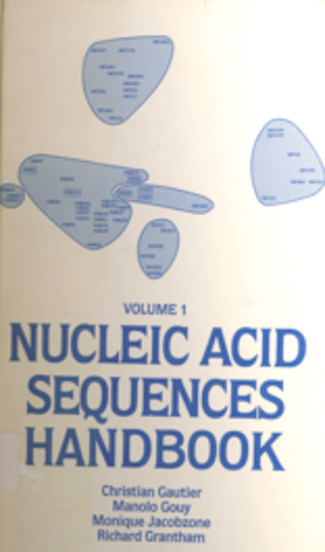
\includegraphics[width=\marginparwidth]{../figs/acnucbook1}\\
\tiny{Cover of ACNUC book vol. 1}
}
\marginpar{
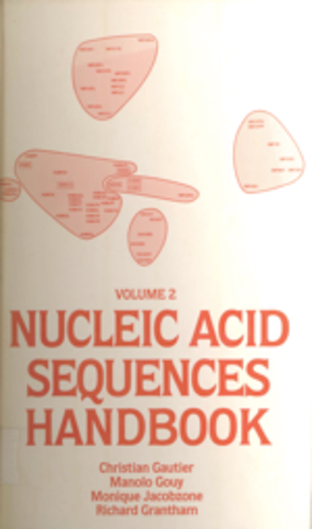
\includegraphics[width=\marginparwidth]{../figs/acnucbook2}\\
\tiny{Cover of ACNUC book vol. 2}
}

ACNUC\footnote{
A contraction of ACides NUCl{\'e}iques, that is \emph{NUCleic ACids}
in french (\url{http://pbil.univ-lyon1.fr/databases/acnuc/acnuc.html})}
was first a database of nucleic acids developed in the early
80's in the same lab (Lyon, France) that issued \seqinr{}. ACNUC was first published
as a printed book in two volumes \cite{GautierC1982a, GautierC1982b}
whose covers are reproduced in margin there. At about the same time, two
other databases were created, one in the USA (GenBank,
at Los Alamos and now managed by the NCBI\footnote{National Center for Biotechnology Information}), 
and another one in Germany
(created in K{\"o}ln by K. St{\"u}ber). To avoid duplication of efforts at the
european level, a single repository database was initiated in Germany yielding
the EMBL\footnote{European Molecular Biology Laboratory} database that moved from K{\"o}ln
to Heidelberg, and then to its current location at the EBI\footnote{European Bioinformatic
Institute} near Cambridge. The DDBJ\footnote{DNA Data Bank of Japan} started
in 1986 at the NIG\footnote{National Institute of Genetics} in Mishima. These three
main repository DNA databases are now collaborating to maintain the INSD\footnote{
International Nucleotide Sequence Database (\url{http://www.insdc.org/})} 
and are sharing data on a daily basis.


The sequences present in the ACNUC books \cite{GautierC1982a, GautierC1982b} were all
the published nucleic acid sequences of about 150 or more continuous
unambiguous nucleotides up to May or June 1981 from the journal given in
table \ref{JournalACNUC}.

\begin{table}[ht]
\begin{scriptsize}
\begin{center}
\begin{tabular}{l}
\hline
\hline
Journal name\\
\hline
\textit{Biochimie}\\
\textit{Biochemistry (ACS)}\\
\textit{Cell}\\
\textit{Comptes Rendus de l'Acad{\'e}mie des Sciences, Paris}\\
\textit{European Journal of Biochemistry}\\
\textit{FEBS Letters}\\
\textit{Gene}\\
\textit{Journal of Bacteriology}\\
\textit{Journal of Biological Chemistry}\\
\textit{Journal of Molecular Biology}\\
\textit{Molecular and General Genetics}\\
\textit{Nature}\\
\textit{Nucleic Acids Research}\\
\textit{Proceedings of the National Academy of Sciences of the United States of America}\\
\textit{Science}\\
\hline
\hline
\end{tabular}
\caption{The list of journals that were manually scanned for nucleic sequences that
were included in the ACNUC books \cite{GautierC1982a, GautierC1982b}}
\label{JournalACNUC}
\end{center}
\end{scriptsize}
\end{table}


The total number of base pair was 526,506 in the two books. They were about 4.5 cm
width. We can then compute of much place would it take to print the last GenBank
release with the same format as the ACNUC book: 
\marginpar{
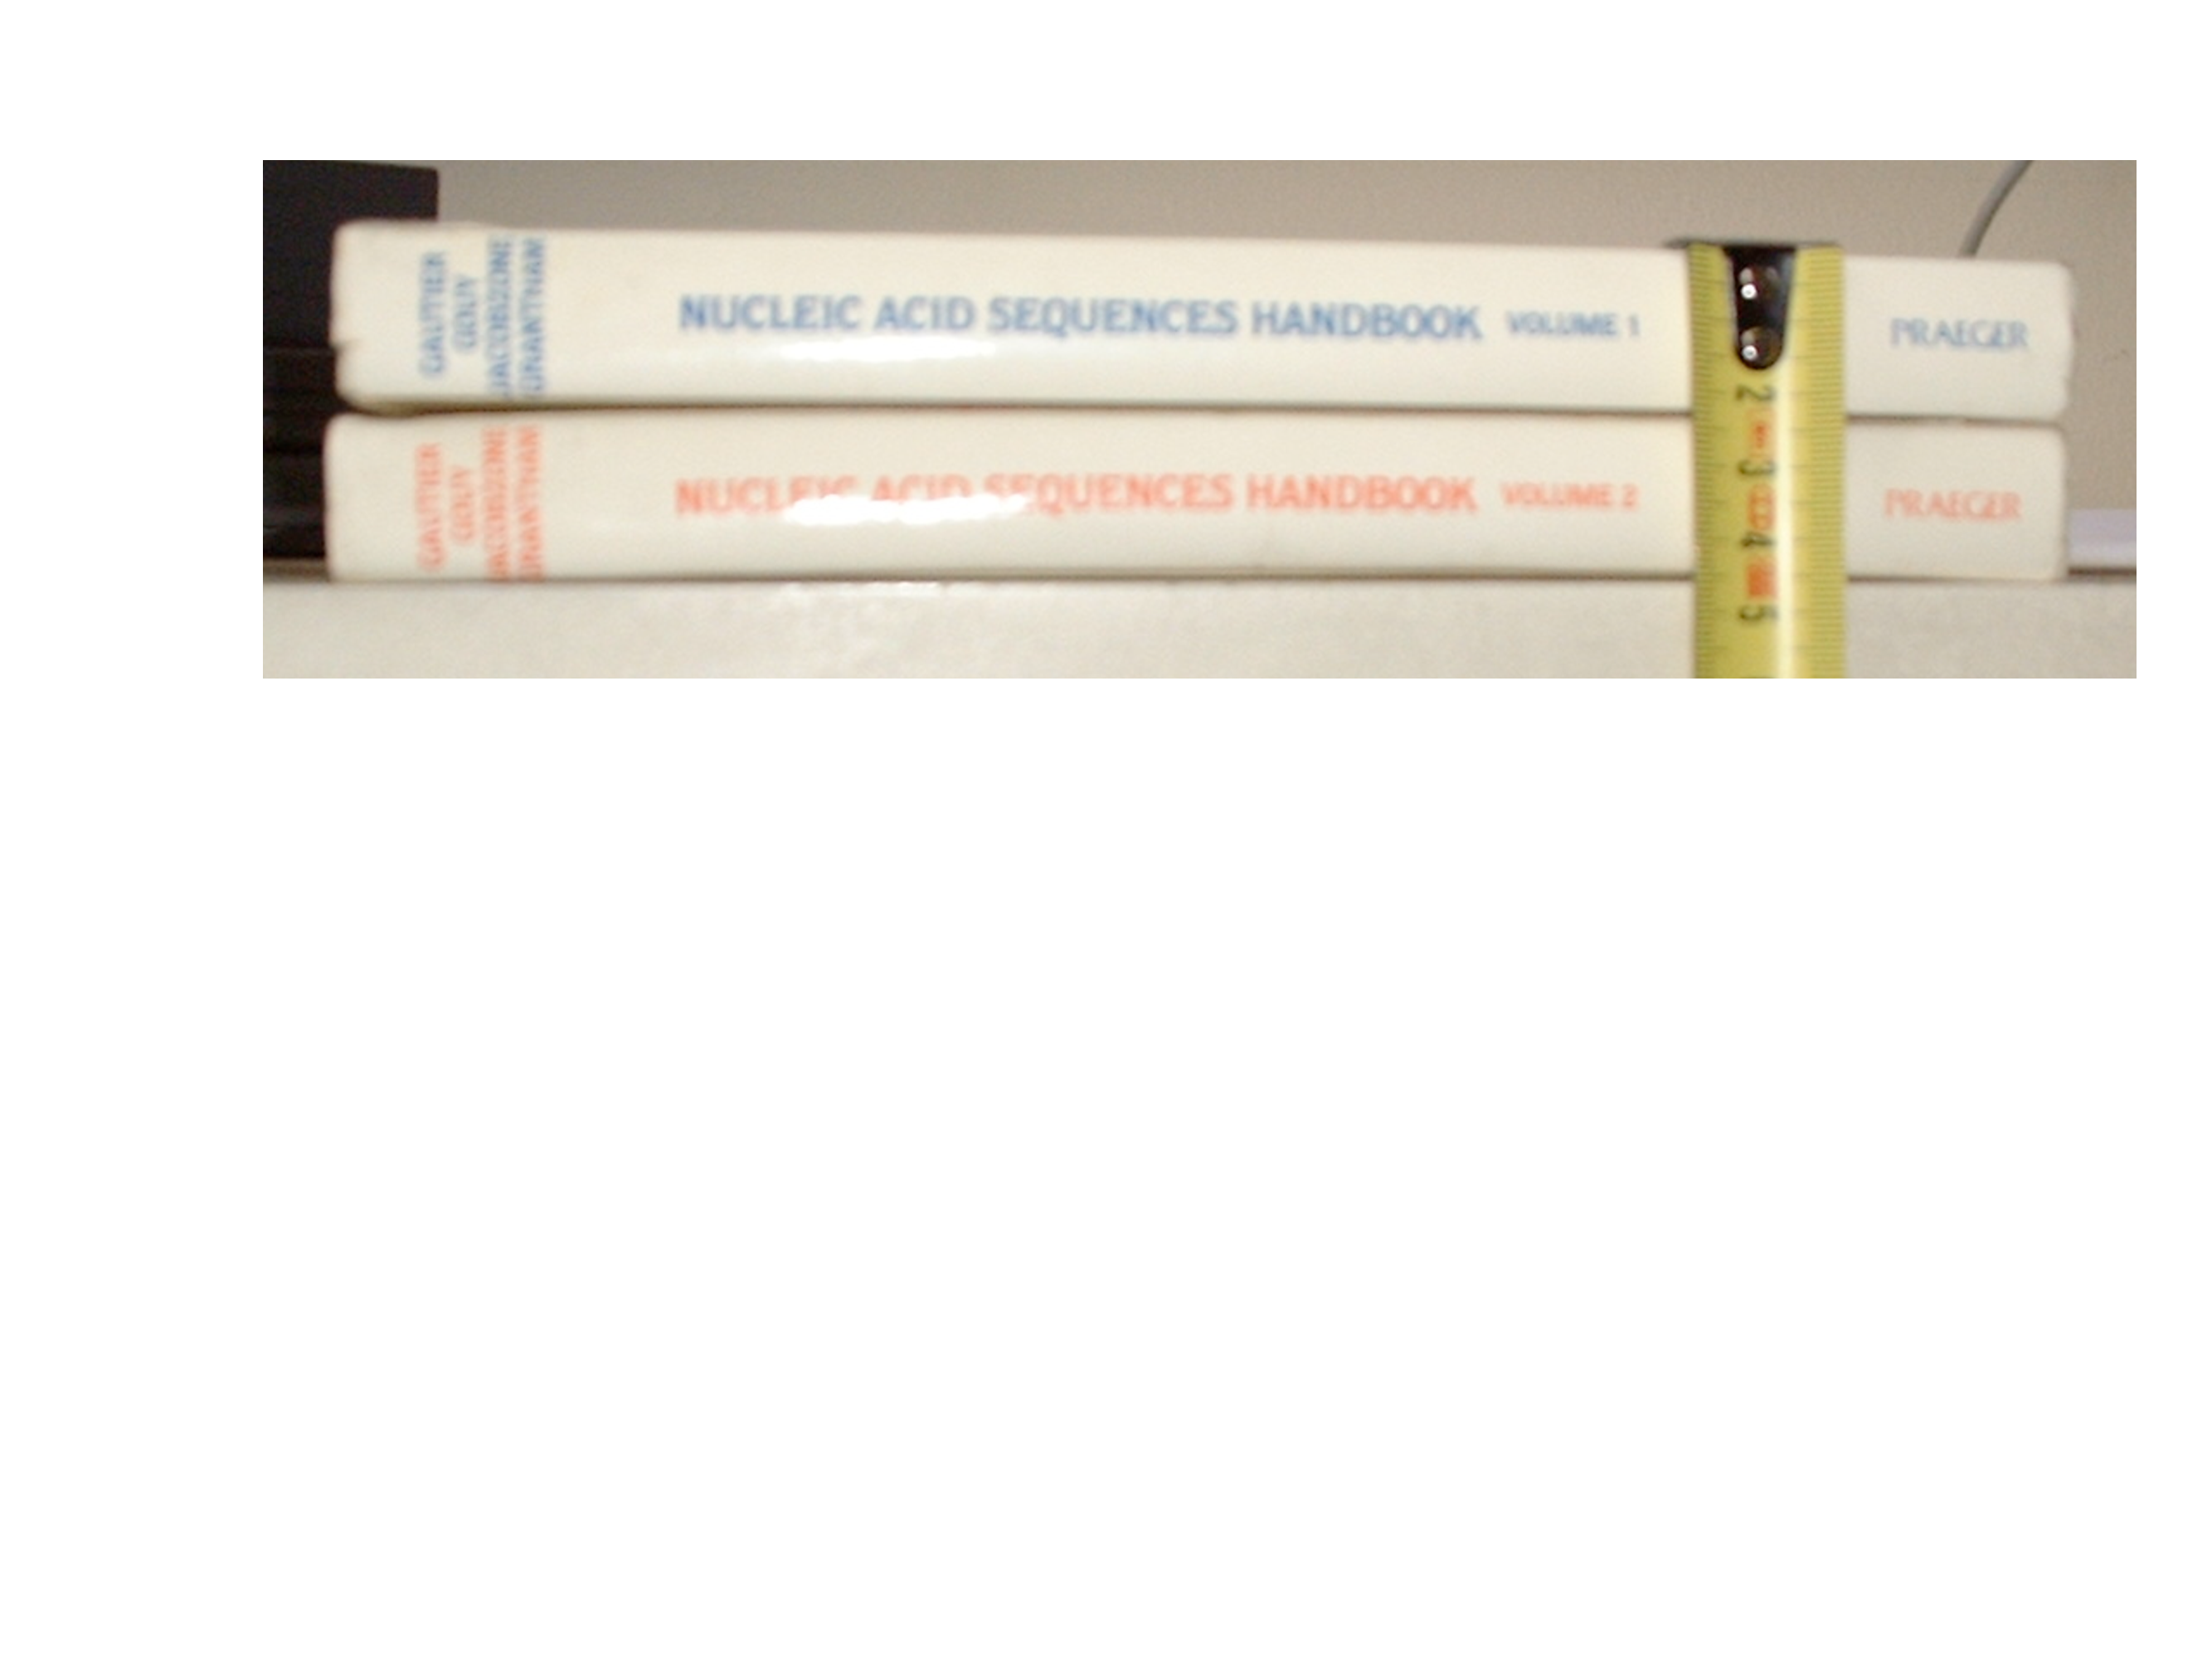
\includegraphics[width=\marginparwidth]{../figs/acnucbook12}\\
\tiny{ACNUC books are about 4.5 cm width}
}

\begin{Schunk}
\begin{Sinput}
 acnucbooksize <- 4.5
 acnucbp <- 526506
 mybank <- choosebank("genbank")
 closebank()
 mybank$details
\end{Sinput}
\begin{Soutput}
[1] "             ****     ACNUC Data Base Content      ****                         "
[2] "          GenBank Rel. 165 (15 April 2008) Last Updated: May 12, 2008"           
[3] "90,620,951,454 bases; 87,387,352 sequences; 5,153,479 subseqs; 508,578 refers."  
[4] "Software by M. Gouy, Lab. Biometrie et Biologie Evolutive, Universite Lyon I "   
\end{Soutput}
\begin{Sinput}
 bpbk <- unlist(strsplit(mybank$details[3], split = " "))[1]
 bpbk
\end{Sinput}
\begin{Soutput}
[1] "90,620,951,454"
\end{Soutput}
\begin{Sinput}
 bpbk <- as.numeric(paste(unlist(strsplit(bpbk, split = ",")), 
     collapse = ""))
 widthcm <- acnucbooksize * bpbk/acnucbp
 (widthkm <- widthcm/10^5)
\end{Sinput}
\begin{Soutput}
[1] 7.745292
\end{Soutput}
\end{Schunk}

It would be about 7.7
kilometer long in ACNUC book format to print GenBank today (\today). As a
matter of comparison, our local universitary library buiding\footnote{
Universit� de Lyon, F-69000, Lyon ; Universit� Lyon 1 ; 
Biblioth$\grave{\mathrm{e}}$que Universitaire Sciences,
18-25-27 Avenue Claude BERNARD,
F-69622, Villeurbanne, France.
} contains about
4 km of books and journals.
\marginpar{
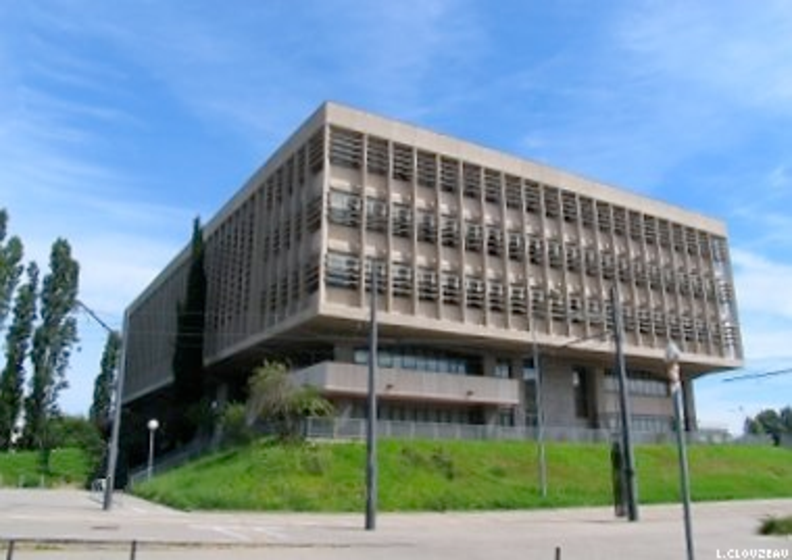
\includegraphics[width=\marginparwidth]{../figs/libraryBuilding}\\
\tiny{Our local library building in 2007 has a capacity of about
4 linear km of journals. That wouldn't be enough to store a printed
version of GenBank. Picture by Lionel Clouzeau.}
}
\section{About R and CRAN}

\Rlogo{} \cite{R, RfromR} is a \emph{libre} language and environment for statistical computing and graphics 
which provides a wide variety of statistical and graphical techniques: linear and 
nonlinear modelling, statistical tests, time series analysis, classification, clustering, etc. 
Please consult the \Rlogo{} project homepage at \texttt{http://www.R-project.org/} for 
further information. 


The Comprehensive \Rlogo{} Archive Network, CRAN, is a network of servers 
around the world that store identical, up-to-date, versions of code and documentation 
for R. At compilation time of this document, there were
52 
mirrors available 
from 32 countries.
Please use the CRAN mirror nearest to you to minimize network load, they are
listed at \texttt{http://cran.r-project.org/mirrors.html}, and can be directly
selected with the function \texttt{chooseCRANmirror()}.

\section{About this document}

In the terminology of the \Rlogo{} project \cite{R, RfromR}, this document 
is a package \emph{vignette}, which means that all code outputs present 
here were actually obtained by runing them.
The examples given thereafter were run under \texttt{R version 2.8.0 Under development (unstable) (2008-05-11 r45672)}
on Mon May 12 17:50:47 2008 with Sweave \cite{Sweave}. There is a section at the end of
each chapter called \textbf{Session Informations} that gives details about
packages and package versions that were involved\footnote{
Previous versions of \Rlogo{} and packages are available on CRAN mirrors,
for instance at \url{http://cran.univ-lyon1.fr/src/contrib/Archive}.
}.
The last compiled version of this document is distributed along with the \seqinr{}
package in the \texttt{/doc} folder. Once \seqinr{} has been installed, the
full path to the package is given by the following \Rlogo{} code :

\begin{Schunk}
\begin{Sinput}
 .find.package("seqinr")
\end{Sinput}
\begin{Soutput}
[1] "/Users/lobry/seqinr.Rcheck/seqinr"
\end{Soutput}
\end{Schunk}


\section{About sequin and \seqinr{}}

Sequin is the well known sofware used to submit sequences to GenBank, \seqinr{}
\cite{seqinr} has definitively no connection with sequin. \seqinr{} is just a shortcut, with
no google hit, for "Sequences in R".

However, as a mnemotechnic tip, you may think about the \seqinr{} package
as the {\bf{R}}eciprocal function of sequin: with sequin you can submit sequences
to Genbank, with \seqinr{} you can {\bf{R}}etrieve sequences from Genbank
(and many other sequence databases). This is
a very good summary of a major functionality of the \seqinr{} package: to
provide an efficient access to sequence databases under R.

\section{About getting started}

You need a computer connected to the Internet. First, install \Rlogo{} on your computer.
There are distributions for Linux, Mac and Windows users
on the CRAN (\texttt{http://cran.r-project.org}). Then, install the \texttt{ape}, 
\texttt{ade4} and \texttt{seqinr} packages. This can be done directly in an \Rlogo{} console
with for instance the command \texttt{install.packages("seqinr")}. 
Last, load the \seqinr{} package with:

\begin{Schunk}
\begin{Sinput}
library(seqinr)
\end{Sinput}
\end{Schunk}

The command \texttt{lseqinr()} lists all what is defined in the package \seqinr{}:

\begin{Schunk}
\begin{Sinput}
 lseqinr()[1:9]
\end{Sinput}
\begin{Soutput}
[1] "AAstat"      "EXP"         "GC"          "GC1"         "GC2"        
[6] "GC3"         "GCpos"       "SEQINR.UTIL" "a"          
\end{Soutput}
\end{Schunk}

We have printed here only the first 9 entries because they are too numerous.
To get help on a specific function, say \texttt{aaa()}, just prefix its name
with a question mark, as in \texttt{?aaa} and press enter.

\section{About running R in batch mode}

Although \Rlogo{} is usually run in an interactive mode, some data pre-processing 
and analyses could be too long. You can run your \Rlogo{} code in batch mode
in a shell with a command that typically looks like :

\begin{verbatim}
unix$ R CMD BATCH input.R results.out &
\end{verbatim}

where \texttt{input.R} is a text file with the \Rlogo{} code you want to run and
\texttt{results.out} a text file to store the outputs. Note that in batch mode,
the graphical user interface is not active so that some graphical devices 
(\textit{e.g.} \texttt{x11}, \texttt{jpeg}, \texttt{png}) are not
available (see the R FAQ \cite{RFAQ} for further details).

It's worth noting that \Rlogo{} uses the XDR representation of binary objects in binary saved files, 
and these are portable across all \Rlogo{} platforms. The \texttt{save()} and \texttt{load()}
functions are very efficient (because of their binary nature) for saving and restoring any 
kind of \Rlogo{} objects, in a platform independent way. To give a striking real example, at a given time
on a given platform, it was about $4$ minutes long to import a numeric table with 70000 lines and 64 columns
with the defaults settings of the \texttt{read.table()} function. Turning it into binary format,
it was then about $8$ \emph{seconds} to restore it with the \texttt{load()} function.
It is therefore advisable in the \texttt{input.R} batch file to save important data or
results (with something like \texttt{save(mybigdata, file = "mybigdata.RData")})
so as to be able to restore them later efficiently in the interactive mode (with something
like \texttt{load("mybigdata.RData")}).


\section{About the learning curve}

\subsection*{Introduction}

If you are used to work with a purely graphical user interface, you may feel frustrated in the
beginning of the learning process because apparently simple things are not so easily
obtained (\textit{ce n'est que le premier pas qui co{\^{u}te} !}).
In the long term, however, you are a winner for the following reasons.

\subsection{Wheel (the)}

Do not re-invent (there's a patent \cite{wheel} on it anyway).
At the compilation time of this document there were 
1321
contributed packages available. Even if you don't want to be spoon-feed 
\textit{{\`a} bouche ouverte}, 
it's not a bad
idea to look around there just to check what's going on in your own application field.
Specialists all around the world are there.

\subsection{Hotline}

There is a very reactive discussion list to help you, just make sure to
read the posting guide there: \url{http://www.R-project.org/posting-guide.html}
before posting. Because of the high traffic on this list, we strongly suggest to answer \emph{yes} at the
question \emph{Would you like to receive list mail batched in a daily  digest?} when
subscribing at \url{https://stat.ethz.ch/mailman/listinfo/r-help}. Some \textit{bons mots}
from the list are archived in the \Rlogo{}~\texttt{fortunes} package.

\subsection{Automation} 
Consider the 178 pages of figures in the additional data file 1
(\url{http://genomebiology.com/2002/3/10/research/0058/suppl/S1}) from \cite{lobrysueoka}. 
They were produced in part automatically (with a proprietary
software that is no more maintained) and manually, involving a lot of
tedious and repetitive manipulations (such as italicising species names by hand in subtitles).
In few words, a waste of time. The advantage of the \Rlogo{}~environment is that once you are
happy with the outputs (including graphical outputs) of an analysis for species x, it's very
easy to run the same analysis on n species. 

\subsection{Reproducibility} 
If you do not consider the reproducibility of scientific results
to be a serious problem in practice, then the paper by Jonathan Buckheit and David Donoho
\cite{repro} is a must read. Molecular data are available in public databases, this is
a necessary but not sufficient condition to allow for the reproducibility of results.
Publishing the \Rlogo{} source code that was used in your analyses is a simple way
to greatly facilitate the reproduction of your results at the expense of no extra cost. 
At the expense of a little extra cost, you may consider to set up a RWeb server
so that even the laziest reviewer may reproduce your results just by clicking on
the "do it again" button in his web browser (\textit{i.e.} without installing any
software on his computer). For an example involving the \seqinr{} pacakage, 
follow this link \url{http://pbil.univ-lyon1.fr/members/lobry/repro/bioinfo04/}
to reproduce on-line the results from \cite{fifine}.

\subsection{Fine tuning} 
You have full control on everything, even the source code
for all functions is available. 
The following graph was specifically designed to illustrate
the first experimental evidence \cite{chargaff} that, on average, we have also [A]=[T] and [C]=[G] 
in single-stranded DNA. These data from Chargaff's lab give the base composition of the L (Ligth) 
strand for 7 bacterial chromosomes.

\setkeys{Gin}{width=0.5\textwidth}
\begin{Schunk}
\begin{Sinput}
 example(chargaff, ask = FALSE)
\end{Sinput}
\end{Schunk}
\includegraphics{../figs/introduction-chargaff}
\setkeys{Gin}{width=0.8\textwidth}

This is a very specialised graph. The filled areas correspond to non-allowed values beause the sum 
of the four bases frequencies cannot exceed 100\%. The white areas correspond to possible values 
(more exactly to the projection from $\mathbb{R}^4$ to the corresponding $\mathbb{R}^2$ 
planes of the region of allowed values). The lines correspond to the very small subset of allowed 
values for which we have in addition [A]=[T] and [C]=[G]. Points represent observed values in
the $7$ bacterial chromosomes. The whole graph is entirely defined by the code given in the
example of the \texttt{chargaff} dataset (\texttt{?chargaff} to see it).

Another example of highly specialised graph is given by the function \texttt{tablecode()} to
display a genetic code as in textbooks :

\setkeys{Gin}{width=0.6\textwidth}
\begin{Schunk}
\begin{Sinput}
 tablecode()
\end{Sinput}
\end{Schunk}
\includegraphics{../figs/introduction-tablecode1}
\setkeys{Gin}{width=0.8\textwidth}

It's very convenient in practice to have a genetic code at hand, and moreover here,
all genetic code variants are available :

\setkeys{Gin}{width=0.6\textwidth}
\begin{Schunk}
\begin{Sinput}
 tablecode(numcode = 2)
\end{Sinput}
\end{Schunk}
\includegraphics{../figs/introduction-tablecode2}
\setkeys{Gin}{width=0.8\textwidth}

As from \seqinr{} 1.0-4, it is possible to export the table of a genetic code into a \LaTeX~document,
for instance table \ref{../tables/code3.tex} and table \ref{../tables/code4.tex} were automatically generated with the following \Rlogo{} code:

\begin{Schunk}
\begin{Sinput}
 tablecode(numcode = 3, latexfile = "../tables/code3.tex", 
     size = "small")
 tablecode(numcode = 4, latexfile = "../tables/code4.tex", 
     size = "small")
\end{Sinput}
\end{Schunk}

\begin{table}
\begin{center}
{\small
\begin{tabular}{*{13}{l}}
\hline
\\
TTT & Phe &  &
TCT & Ser &  &
TAT & Tyr &  &
TGT & Cys &  &
\\
TTC & Phe &  &
TCC & Ser &  &
TAC & Tyr &  &
TGC & Cys &  &
\\
TTA & Leu &  &
TCA & Ser &  &
TAA & Stp &  &
TGA & Trp &  &
\\
TTG & Leu &  &
TCG & Ser &  &
TAG & Stp &  &
TGG & Trp &  &
\\
\\
CTT & Thr &  &
CCT & Pro &  &
CAT & His &  &
CGT & Arg &  &
\\
CTC & Thr &  &
CCC & Pro &  &
CAC & His &  &
CGC & Arg &  &
\\
CTA & Thr &  &
CCA & Pro &  &
CAA & Gln &  &
CGA & Arg &  &
\\
CTG & Thr &  &
CCG & Pro &  &
CAG & Gln &  &
CGG & Arg &  &
\\
\\
ATT & Ile &  &
ACT & Thr &  &
AAT & Asn &  &
AGT & Ser &  &
\\
ATC & Ile &  &
ACC & Thr &  &
AAC & Asn &  &
AGC & Ser &  &
\\
ATA & Met &  &
ACA & Thr &  &
AAA & Lys &  &
AGA & Arg &  &
\\
ATG & Met &  &
ACG & Thr &  &
AAG & Lys &  &
AGG & Arg &  &
\\
\\
GTT & Val &  &
GCT & Ala &  &
GAT & Asp &  &
GGT & Gly &  &
\\
GTC & Val &  &
GCC & Ala &  &
GAC & Asp &  &
GGC & Gly &  &
\\
GTA & Val &  &
GCA & Ala &  &
GAA & Glu &  &
GGA & Gly &  &
\\
GTG & Val &  &
GCG & Ala &  &
GAG & Glu &  &
GGG & Gly &  &
\\
\\
\hline
\end{tabular}
\caption{Genetic code number 3: yeast.mitochondrial.}
\label{../tables/code3.tex}
}
\end{center}
\end{table}

\begin{table}
\begin{center}
{\small
\begin{tabular}{*{13}{l}}
\hline
\\
TTT & Phe &  &
TCT & Ser &  &
TAT & Tyr &  &
TGT & Cys &  &
\\
TTC & Phe &  &
TCC & Ser &  &
TAC & Tyr &  &
TGC & Cys &  &
\\
TTA & Leu &  &
TCA & Ser &  &
TAA & Stp &  &
TGA & Trp &  &
\\
TTG & Leu &  &
TCG & Ser &  &
TAG & Stp &  &
TGG & Trp &  &
\\
\\
CTT & Leu &  &
CCT & Pro &  &
CAT & His &  &
CGT & Arg &  &
\\
CTC & Leu &  &
CCC & Pro &  &
CAC & His &  &
CGC & Arg &  &
\\
CTA & Leu &  &
CCA & Pro &  &
CAA & Gln &  &
CGA & Arg &  &
\\
CTG & Leu &  &
CCG & Pro &  &
CAG & Gln &  &
CGG & Arg &  &
\\
\\
ATT & Ile &  &
ACT & Thr &  &
AAT & Asn &  &
AGT & Ser &  &
\\
ATC & Ile &  &
ACC & Thr &  &
AAC & Asn &  &
AGC & Ser &  &
\\
ATA & Ile &  &
ACA & Thr &  &
AAA & Lys &  &
AGA & Arg &  &
\\
ATG & Met &  &
ACG & Thr &  &
AAG & Lys &  &
AGG & Arg &  &
\\
\\
GTT & Val &  &
GCT & Ala &  &
GAT & Asp &  &
GGT & Gly &  &
\\
GTC & Val &  &
GCC & Ala &  &
GAC & Asp &  &
GGC & Gly &  &
\\
GTA & Val &  &
GCA & Ala &  &
GAA & Glu &  &
GGA & Gly &  &
\\
GTG & Val &  &
GCG & Ala &  &
GAG & Glu &  &
GGG & Gly &  &
\\
\\
\hline
\end{tabular}
\caption{Genetic code number 4: protozoan.mitochondrial+mycoplasma.}
\label{../tables/code4.tex}
}
\end{center}
\end{table}


The tables were then inserted in the \LaTeX~file with:
\begin{verbatim}
\begin{table}
\begin{center}
{\small
\begin{tabular}{*{13}{l}}
\hline
\\
TTT & Phe &  &
TCT & Ser &  &
TAT & Tyr &  &
TGT & Cys &  &
\\
TTC & Phe &  &
TCC & Ser &  &
TAC & Tyr &  &
TGC & Cys &  &
\\
TTA & Leu &  &
TCA & Ser &  &
TAA & Stp &  &
TGA & Trp &  &
\\
TTG & Leu &  &
TCG & Ser &  &
TAG & Stp &  &
TGG & Trp &  &
\\
\\
CTT & Thr &  &
CCT & Pro &  &
CAT & His &  &
CGT & Arg &  &
\\
CTC & Thr &  &
CCC & Pro &  &
CAC & His &  &
CGC & Arg &  &
\\
CTA & Thr &  &
CCA & Pro &  &
CAA & Gln &  &
CGA & Arg &  &
\\
CTG & Thr &  &
CCG & Pro &  &
CAG & Gln &  &
CGG & Arg &  &
\\
\\
ATT & Ile &  &
ACT & Thr &  &
AAT & Asn &  &
AGT & Ser &  &
\\
ATC & Ile &  &
ACC & Thr &  &
AAC & Asn &  &
AGC & Ser &  &
\\
ATA & Met &  &
ACA & Thr &  &
AAA & Lys &  &
AGA & Arg &  &
\\
ATG & Met &  &
ACG & Thr &  &
AAG & Lys &  &
AGG & Arg &  &
\\
\\
GTT & Val &  &
GCT & Ala &  &
GAT & Asp &  &
GGT & Gly &  &
\\
GTC & Val &  &
GCC & Ala &  &
GAC & Asp &  &
GGC & Gly &  &
\\
GTA & Val &  &
GCA & Ala &  &
GAA & Glu &  &
GGA & Gly &  &
\\
GTG & Val &  &
GCG & Ala &  &
GAG & Glu &  &
GGG & Gly &  &
\\
\\
\hline
\end{tabular}
\caption{Genetic code number 3: yeast.mitochondrial.}
\label{../tables/code3.tex}
}
\end{center}
\end{table}

\begin{table}
\begin{center}
{\small
\begin{tabular}{*{13}{l}}
\hline
\\
TTT & Phe &  &
TCT & Ser &  &
TAT & Tyr &  &
TGT & Cys &  &
\\
TTC & Phe &  &
TCC & Ser &  &
TAC & Tyr &  &
TGC & Cys &  &
\\
TTA & Leu &  &
TCA & Ser &  &
TAA & Stp &  &
TGA & Trp &  &
\\
TTG & Leu &  &
TCG & Ser &  &
TAG & Stp &  &
TGG & Trp &  &
\\
\\
CTT & Leu &  &
CCT & Pro &  &
CAT & His &  &
CGT & Arg &  &
\\
CTC & Leu &  &
CCC & Pro &  &
CAC & His &  &
CGC & Arg &  &
\\
CTA & Leu &  &
CCA & Pro &  &
CAA & Gln &  &
CGA & Arg &  &
\\
CTG & Leu &  &
CCG & Pro &  &
CAG & Gln &  &
CGG & Arg &  &
\\
\\
ATT & Ile &  &
ACT & Thr &  &
AAT & Asn &  &
AGT & Ser &  &
\\
ATC & Ile &  &
ACC & Thr &  &
AAC & Asn &  &
AGC & Ser &  &
\\
ATA & Ile &  &
ACA & Thr &  &
AAA & Lys &  &
AGA & Arg &  &
\\
ATG & Met &  &
ACG & Thr &  &
AAG & Lys &  &
AGG & Arg &  &
\\
\\
GTT & Val &  &
GCT & Ala &  &
GAT & Asp &  &
GGT & Gly &  &
\\
GTC & Val &  &
GCC & Ala &  &
GAC & Asp &  &
GGC & Gly &  &
\\
GTA & Val &  &
GCA & Ala &  &
GAA & Glu &  &
GGA & Gly &  &
\\
GTG & Val &  &
GCG & Ala &  &
GAG & Glu &  &
GGG & Gly &  &
\\
\\
\hline
\end{tabular}
\caption{Genetic code number 4: protozoan.mitochondrial+mycoplasma.}
\label{../tables/code4.tex}
}
\end{center}
\end{table}

\end{verbatim}

\subsection{Data as fast moving targets}
 
In research area, data are not always stable. 
Consider figure 1 from \cite{lobrylncs} which is reproduced here in figure \ref{fig1lncs2004}.
Data have been updated since then, but we can re-use  the same \Rlogo{}~code\footnote{
This code was adapted from \url{http://pbil.univ-lyon1.fr/members/lobry/repro/lncs04/}.
}
to update the figure:

\setkeys{Gin}{width=\textwidth}
\begin{Schunk}
\begin{Sinput}
 data <- get.db.growth()
 scale <- 1
 ltymoore <- 1
 date <- data$date
 Nucleotides <- data$Nucleotides
 Month <- data$Month
 plot.default(date, log10(Nucleotides), main = "Update of Fig. 1 from Lobry (2004) LNCS, 3039:679:\nThe exponential growth of genome sequence data", 
     xlab = "Year", ylab = "Log10 number of nucleotides", pch = 19, 
     las = 1, cex = scale, cex.axis = scale, cex.lab = scale)
 abline(lm(log10(Nucleotides) ~ date), lwd = 2)
 lm1 <- lm(log(Nucleotides) ~ date)
 mu <- lm1$coef[2]
 dbt <- log(2)/mu
 dbt <- 12 * dbt
 x <- mean(date)
 y <- mean(log10(Nucleotides))
 a <- log10(2)/1.5
 b <- y - a * x
 lm10 <- lm(log10(Nucleotides) ~ date)
 for (i in seq(-10, 10, by = 1)) if (i != 0) abline(coef = c(b + 
     i, a), col = "black", lty = ltymoore)
\end{Sinput}
\end{Schunk}
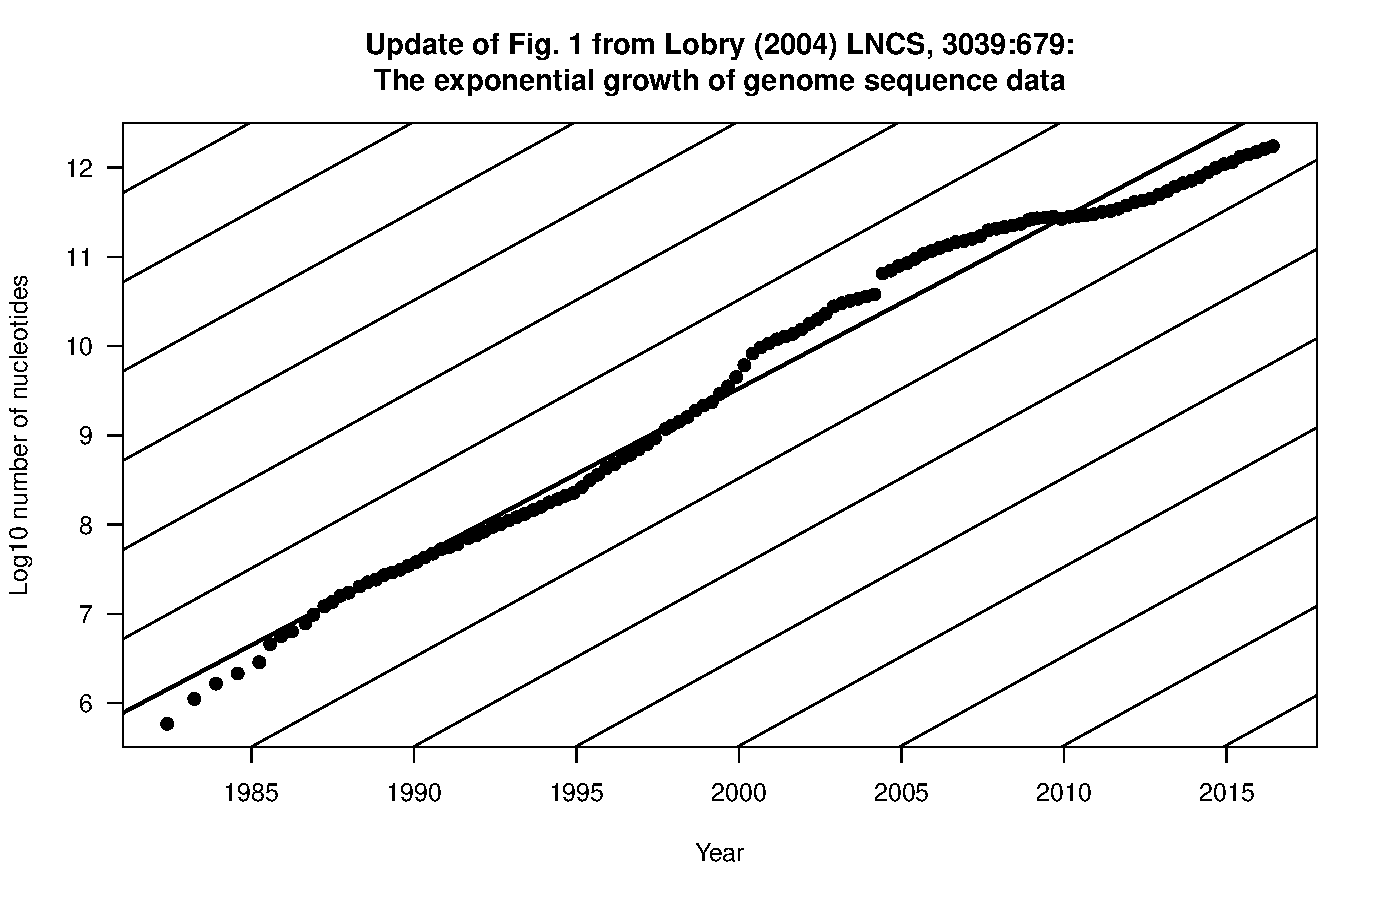
\includegraphics{../figs/introduction-dbg}
\setkeys{Gin}{width=0.8\textwidth}


The doubling time is now 16.6 months.


\begin{figure}
\begin{center}
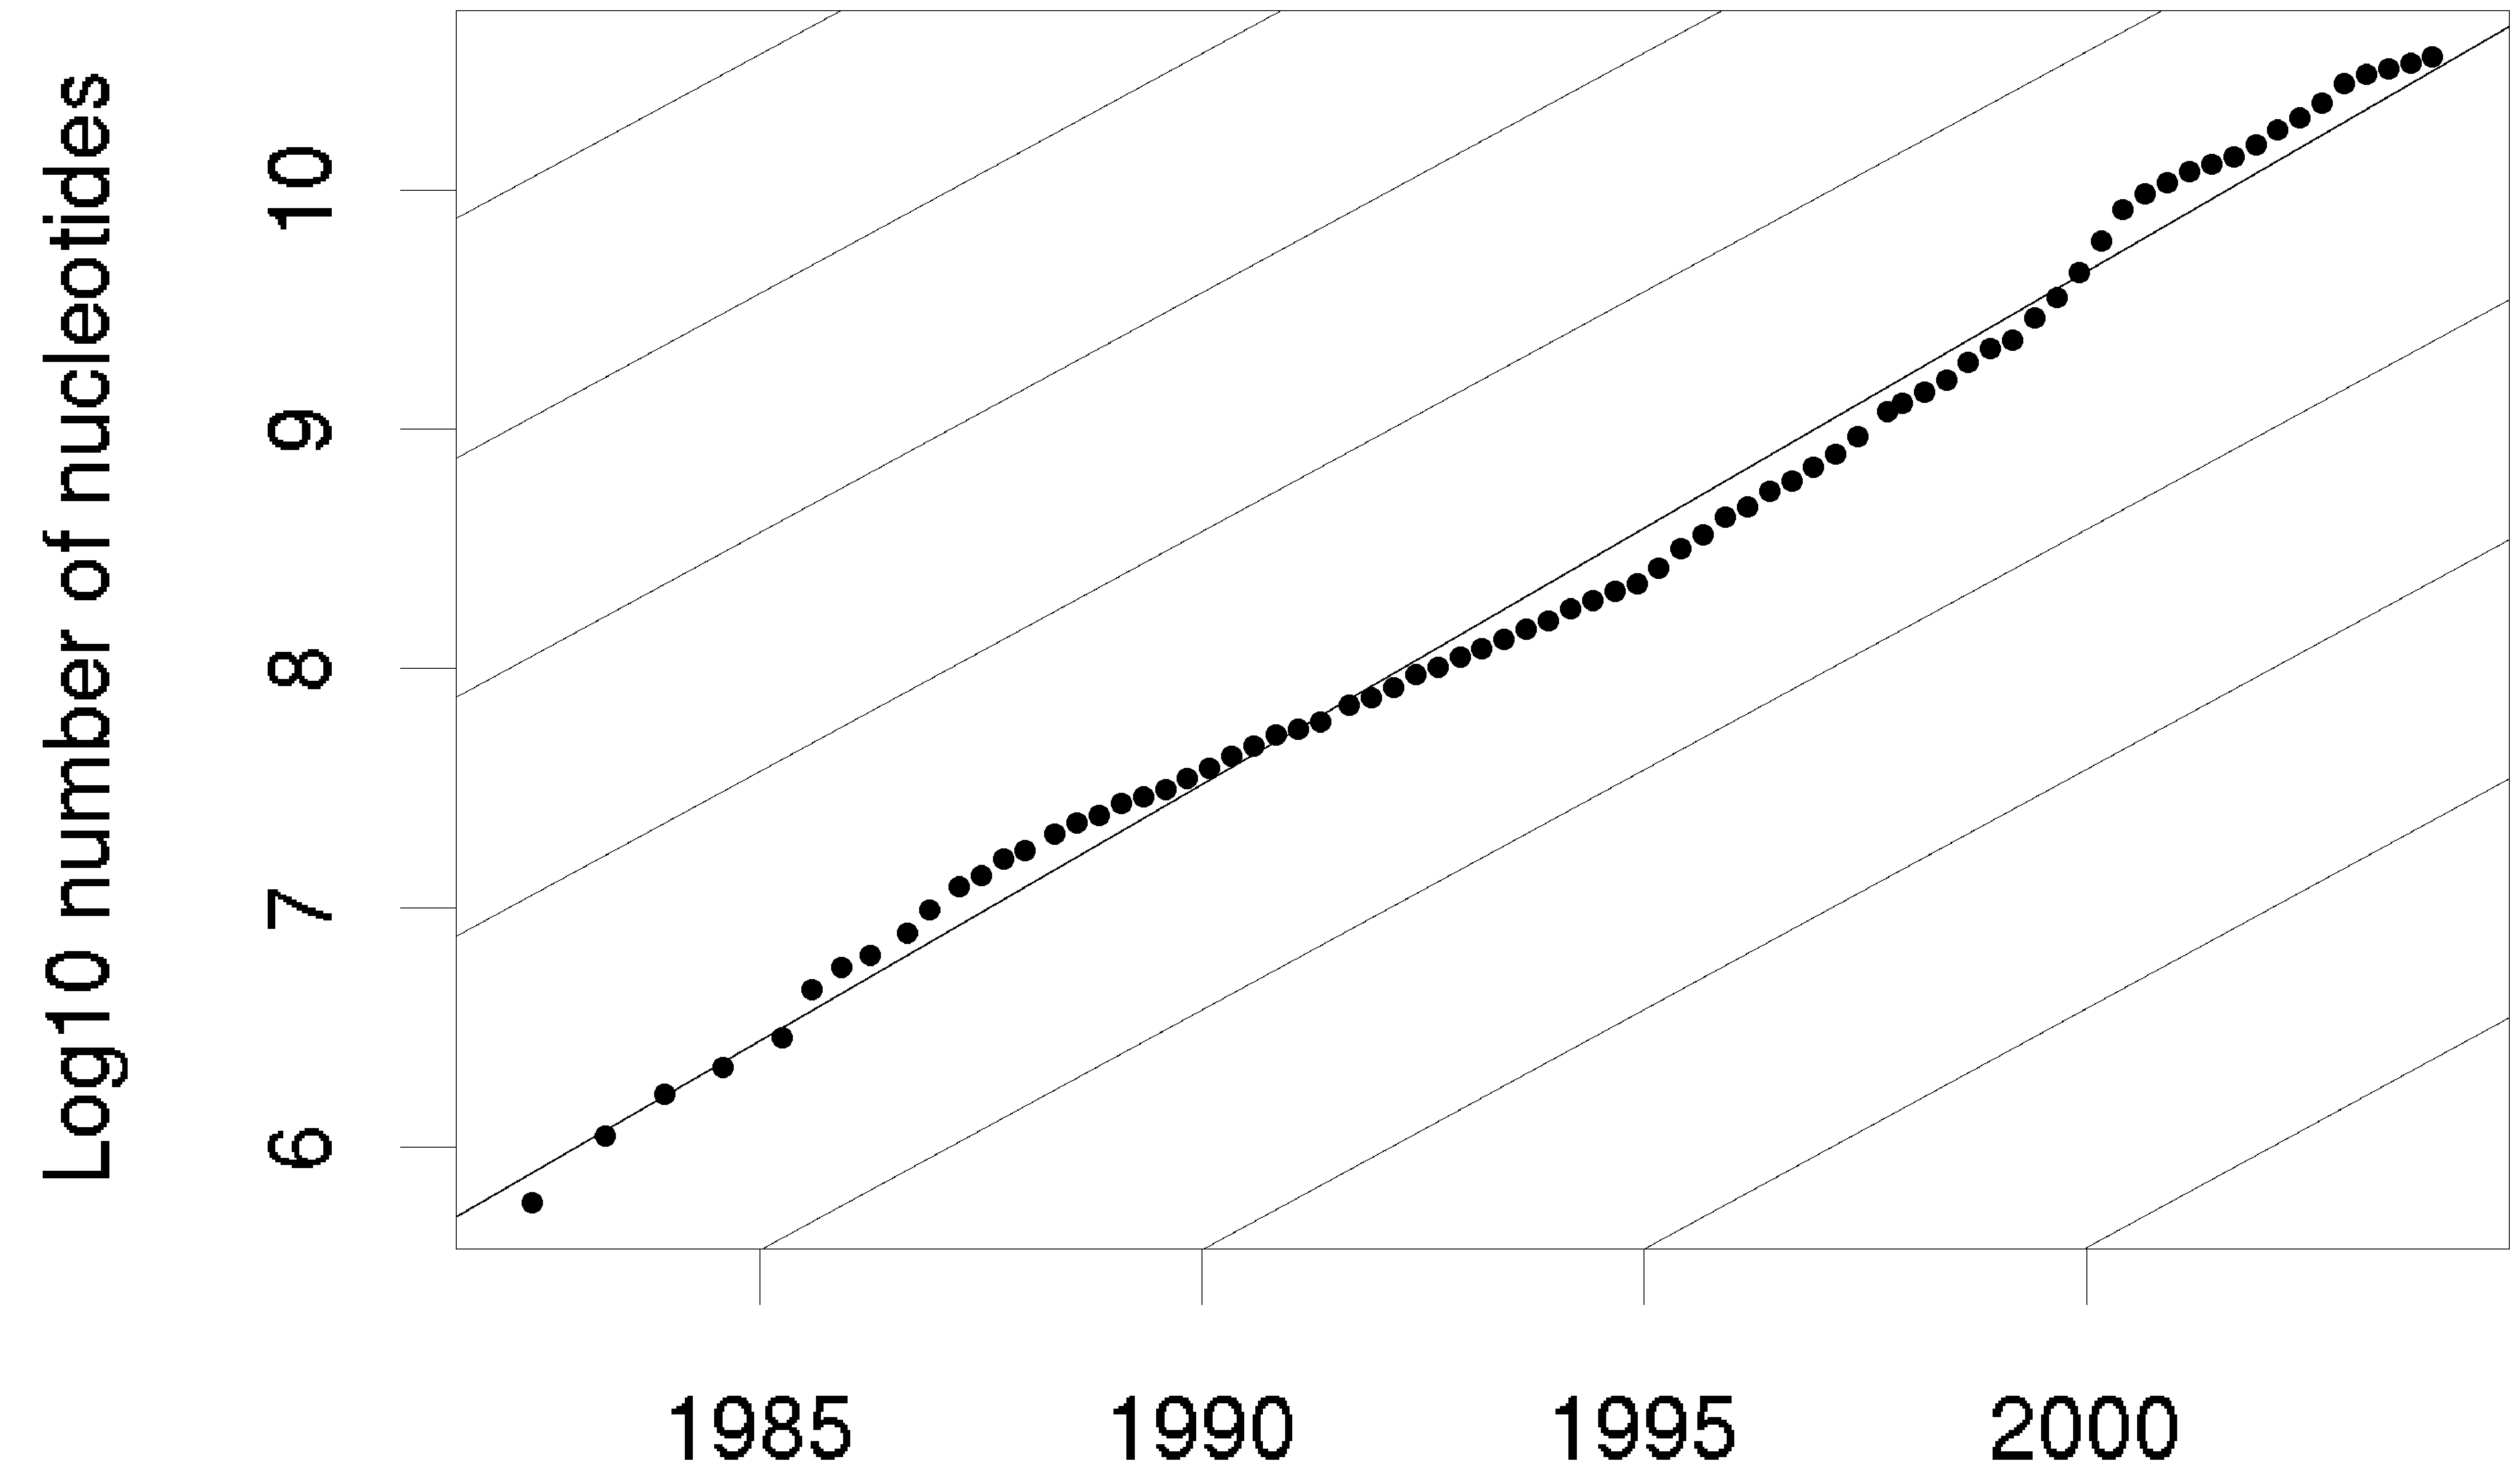
\includegraphics[width=\textwidth]{../figs/fig1lncs2004}
\end{center}
\caption{Screenshot of figure 1 from \cite{lobrylncs}.
The exponential growth of genomic sequence data mimics Moore's law.
The source of data is the december 2003 release note (realnote.txt) from the EMBL database
available at \protect\url{http://www.ebi.ac.uk/}. External lines correspond to what would be expected with
a doubling time of 18 months. The central line through points is the best least square fit,
corresponding to a doubling time of 16.9 months.}
\label{fig1lncs2004}
\end{figure}

\subsection{\texttt{Sweave()} and \texttt{xtable()}}

For \LaTeX~users, it's
worth mentioning the fantastic tool contributed by Friedrich Leish \cite{Sweave}
called \texttt{Sweave()} that allows for the automatic insertion
of \Rlogo{}~outputs (including graphics) in a \LaTeX~document. In the same spirit, there
is a package called \texttt{xtable} \cite{xtable} to coerce \Rlogo{}~data into \LaTeX~tables.


\section*{Session Informations}

This part was compiled under the following \Rlogo{}~environment:

\begin{itemize}
  \item R version 2.8.0 Under development (unstable) (2008-05-11 r45672), \verb|i386-apple-darwin8.8.2|
  \item Locale: \verb|C|
  \item Base packages: base, datasets, grDevices, graphics, methods,
    stats, utils
  \item Other packages: MASS~7.2-42, ade4~1.4-7, ape~2.2,
    nlme~3.1-88, seqinr~1.1-6, xtable~1.5-2
  \item Loaded via a namespace (and not attached): grid~2.8.0,
    lattice~0.17-7, tools~2.8.0
\end{itemize}
There were two compilation steps:

\begin{itemize}
  \item \Rlogo{} compilation time was: Mon May 12 17:50:52 2008
  \item \LaTeX{} compilation time was: \today
\end{itemize}

% END - DO NOT REMOVE THIS LINE

%%%%%%%%%%%%  BIBLIOGRAPHY %%%%%%%%%%%%%%%%%
\clearpage
\addcontentsline{toc}{section}{References}
\bibliographystyle{plain}
\bibliography{../config/book}
\end{document}
